\documentclass[]{article}
% includes
\usepackage{amsmath}
\usepackage{amsthm}
\usepackage{amssymb}
\usepackage{authblk}
\usepackage{mathtools}
\usepackage{makecell}
\usepackage{physics}
\usepackage{hyperref}
\usepackage{bm}\newcommand{\ind}{\bm{1}}
\usepackage{multirow}
\usepackage[table]{xcolor}
\usepackage{booktabs}
\usepackage[utf8]{inputenc}
\usepackage{adjustbox}
\usepackage{caption}\captionsetup[table]{skip=1em}
\usepackage{rotating}
\usepackage{graphicx}
\graphicspath{{fig/}}
\usepackage[margin=3cm]{geometry}

% definitions
\DeclarePairedDelimiter{\floor}{\lfloor}{\rfloor}
\DeclarePairedDelimiter{\ceil}{\lceil}{\rceil}
\DeclareUnicodeCharacter{2713}{\checkmark}
\setlength{\parskip}{1em}
%\DeclarePairedDelimiter{\floor}{\lfloor}{\rfloor}
\DeclarePairedDelimiter{\ceil}{\lceil}{\rceil}
\newcommand{\ind}{\mathbbm{1}}

\title{A flexible integer linear programming formulation for scheduling
	clinician on-call service in hospitals}

\author[a, b]{David Landsman}
\author[a]{Huiting Ma}
\author[a]{Jesse Knight}
\author[c]{Kevin Gough}
\author[a, c, d, e]{Sharmistha Mishra}

\renewcommand\Affilfont{\itshape\small}
\affil[a]{MAP Centre for Urban Health Solutions, Unity Health Toronto, Toronto,
	ON, Canada}
\affil[b]{Department of Computer Science, University of Toronto, Toronto, ON,
	Canada}
\affil[c]{Department of Medicine, Division of Infectious Disease, St.\ Michael's
	Hospital, University of Toronto, Toronto, ON, Canada}
\affil[d]{Institute of Health Policy, Management and Evaluation, Dalla Lana
	School of Public Health, University of Toronto, Toronto, ON, Canada}
\affil[e]{Institute of Medical Sciences, University of Toronto, Toronto, ON,
	Canada}

\begin{document}
	\maketitle
	
	\begin{abstract}
		Scheduling of personnel in a hospital environment is vital to improving the service provided to patients and balancing the workload assigned to clinicians. Many approaches have been tried and successfully applied to generate efficient schedules in such settings. However, due to the computational complexity of the scheduling problem in general, most approaches resort to heuristics to find a non-optimal solution in a reasonable amount of time. We designed an integer linear programming formulation to find an optimal schedule in a clinical division of a hospital. Our formulation mitigates computational complexity issues by maintaining a minimal set of constraints, yet still provides the flexibility necessary to adapt it to a variety of clinical divisions. \\

We then conducted a case study for our approach using data from the Infectious Diseases division at St. Michael's Hospital in Toronto, Canada. We analyzed and compared the results of our approach to manually-created schedules at the hospital, and found improved adherence to departmental constraints and clinician preferences. We used simulated data to examine the sensitivity of the runtime of our linear program for various parameters and observed reassuring results, signifying the practicality and generazability of our approach in different real-world scenarios.
	\end{abstract}
	
	\section{Introduction}\label{sec:introduction}
	Hospital departments provide services where patient needs, and thus the system's demands, often exceed the available supply. In particular, on-call schedules for a fixed number of health-care providers are central to the efficient running of hospitals. Carefully allocated schedules are meant to simultaneously ensure sufficient resources are provided to patients while not overworking clinicians to prevent costly mistakes [ref]. It is common practice for on-call schedules in hospitals to be created manually, yet manually-created schedules are prone to errors and potential for various biases [ref]. First, when there is a large number of clinicians in a single department, or the constraints that need to be satisfied by the department are very complex, a manual method may not provide an optimal schedule. Second, such methods are likely to overlook certain constraints that must be maintained to have an operational department, such as preventing many consecutive work blocks from being assigned or ensuring clinicians are allocated a specific amount of work blocks throughout the year. Third, manual scheduling is often time-consuming for the person developing the schedule. For these reasons, it is important to develop automated methods that can generate optimal schedules that satisfy the given constraints of the hospital department. \\
%For example, it is important that a hospital department allocates its resources, such as the availability of a finite number of clinicians, optimally, to ensure the best possible service for its patients.

Automated methods to optimize schedules have been studied and applied in many industries, including transportation \cite{aickelin_improved_2006, goel_truck_2012, gunther_combined_2010}, manufacturing \cite{al-yakoob_mixed-integer_2007, al-yakoob_column_2008, alfares_simulation_2007}, retail \cite{chapados_retail_2011, nissen_automatic_2010} and military \cite{horn_scheduling_2007, laguna_modeling_2005}. Of special interest to a clinician on-call scheduling problem are the approaches to schedule nurses, who often work in shifts. In the nurse scheduling problem, the goal is to find an optimal assignment of nurses to shifts that satisfies all of the hard constraints, such as hospital regulations, and as many soft constraints as possible, which may include nurse preferences. A wide variety of approaches, including exact and heuristic approaches, have been used to solve the nurse scheduling problem: integer linear programming \cite{azaiez_0-1_2005, trilling_nurse_2006, widyastiti_nurses_2016}, network flows \cite{el_adoly_new_2018}, genetic algorithms \cite{aickelin_exploiting_2000, jan_evolutionary_2000, kawanaka_genetic_2001}, simulated annealing \cite{jaszkiewicz_metaheuristic_1997}, and artificial intelligence \cite{abdennadher_nurse_nodate, li_hybrid_2003}. A comprehensive literature review of these and other methods applied to nurse rostering is presented in \cite{burke_state_2004}. \\

%An extensive literature review of these and other methods is presented by [??]. We will briefly summarize the main ideas of some of these approaches. \\ SM - don't need to introduce that you will do this for this type of paper I think - would do in a thesis chapter though.

Many of the approaches to nurse scheduling were designed to satisfy the requirements of a specific hospital department which causes a large number of variables and constraints to be incorporated into the problem formulation. While these department-specific approaches allow end-users to find precise schedules that satisfy the needs of the department and the preferences of the nurses and clinicians in that department, they are difficult to readily adapt to other departments in the same hospital or other hospitals. % explain why hard to adapt?... what makes their generalizablility/adaptability limited?
Moreover, the large number of variables and constraints also leads to computational complexity issues \cite{goos_complexity_1996}, especially when using exact methods for finding the solution. In this paper, we tackle a version of the nurse scheduling problem arising from a case study of one clinical division, providing two different services simultaneously (general infectious disease (ID) consults; and HIV consults service) at St. Michael's Hospital in Toronto, Canada. Our goal is to (1) present a simple integer linear programming formulations for the scheduling problem as developed for the hospital, and describe the adaptability of the formulation to solving similar problems in other departments; (2) compare the performance of the ILP scheduler to the results of the manual approach; and (3) analyze the robustness of the algorithm in difficult instances of the problem. \\
% present a simple formulation for the problem developed and tested at the hospital after switching from a manual approach to scheduling; and (2) analyze the performance of integer linear programming in solving difficult instances of the problem and compare the results with those of the manual approach; and (3) describe the adaptability of the formulation as a basic framework for solving similar problems in other departments. \\ %make #3 an objective

We begin by describing the problem in Section \ref{sec:problem}, and presenting our ILP formulation in Section \ref{sec:methods}. Next, we compare the results of our formulation to manually-created schedules, and evaluate the performance of the algorithm on simulated data in Section \ref{sec:results}. Finally, we discuss and interpret the results in Section \ref{sec:discussion}. % list the main contents/elements of the paper.
	\section{Problem}\label{sec:problem}
	\subsection{Overview}
At St. Michael's Hospital, the (???) division offers general ID and HIV consultation throughout the whole year, during regular work weeks as well as weekends and holidays. The clinicians in the division typically receive a schedule in advance, outlining their on-call service dates for the full year. In the yearly schedule each clinician is assigned to blocks of regular work weeks, as well as weekends. Each block corresponds to two consecutive work weeks. Apart from long (holiday) weekends, a work week starts on Monday at 8 A.M. and ends on Friday at 5 P.M. Conversely, weekend service starts on Friday at 5 P.M., and goes on until the start of the next work week on Monday at 8 A.M. During the weekend, all clinicians in the department provide both ID and HIV consultation, while during the week some clinicians only provide one of the two services. \\

In order to provide quality service and ensure patients get the best care they can, it is important to prevent under- and over-working of clinicians. Several constraints are placed on the assignments in hopes of preventing such issues. Firstly, each clinician has limits on the number of blocks they can and must work during the year, depending on the type of consultation. For instance, a clinician might have to provide 3-5 blocks of general ID consultation as well as 2-3 blocks of HIV consultation throughout the year. These limits may change from year to year as the number of clinicians in the department changes. Moreover, the schedule does not assign a clinician to work for two blocks or two weekends in a row. It is especially important to prevent over-working during weekends, as the demand for the on-call service increases drastically. Hence, the schedule attempts to distribute both regular and holiday weekends equally among all clinicians. \\

Apart from maintaining a balanced work load among clinicians, the schedule also tries to accommodate their preferences. Clinicians provide their requests for time off ahead of schedule generation so that they can be integrated into the schedule. They are free to specify days, weeks or weekends off, with the understanding that any blocks overlapping with their request will be assigned to a different clinician, if possible. For example, if a clinician only requests Monday and Tuesday off, the schedule will generally avoid assigning the entire block to that clinician. Clinicians also prefer to have their weekend and block assignments close together, so the schedule tries to take this into account when distributing assignments. \\

[...]

\subsection{Mathematical Formulation}
[...] \\

Table \ref{tbl:sets-indices} presents the sets and indices that are used in the definition of the constraints. Table \ref{tbl:variables-constants} presents the constants and variables in the problem.

\begin{table}[h]
	\centering
	\begin{tabular}{ c c l }
		\hline
		set                                  & index & description                       \\ \hline
		$\mathcal{D} = \{1, \ldots, D \}$    & $d$   & services/divisions                \\
		$\mathcal{C} = \{1, \ldots, C \}$    & $c$   & clinicians                        \\
		$\mathcal{B} = \{1, \ldots, B \}$    & $b$   & blocks                            \\
		$\mathcal{W} = \{1, \ldots, W \}$    & $w$   & weekends                          \\
		$\mathcal{L} \subset \mathcal{W}$    &       & long weekends                     \\
		$\mathcal{BR}_c \subset \mathcal{B}$ &       & block requests of clinician $c$   \\
		$\mathcal{WR}_c \subset \mathcal{W}$ &       & weekend requests of clinician $c$
	\end{tabular}
	\caption{Description of sets and indices in the problem}
	\label{tbl:sets-indices}
\end{table}

\begin{table}[h]
	\centering
	\begin{tabular}{ c l }
		\hline
		name                       & description                                                          \\ \hline
		$X_{c, b, d} \in \{0, 1\}$ & assignment of clinician $c$ for division $d$ on block $b$            \\
		$Y_{c, w} \in \{0, 1\}$    & assignment of clinician $c$ on weekend $w$                           \\
		$m_{c, d}$                 & minimum number of blocks clinician $c$ should cover for division $d$ \\
		$M_{c, d}$                 & maximum number of blocks clinician $c$ should cover for division $d$
	\end{tabular}
	\caption{Description of variables and constants in the problem}
	\label{tbl:variables-constants}
\end{table}
	\section{Methods}\label{sec:methods}
	In this section, we present an application of ILP to solve the clinician
scheduling problem presented in Section~\ref{sec:problem}. First, we describe
the sets, indices and variables present in the formulation of the program. We
then convert the constraints given in Table~\ref{tbl:constraint-summary} into
mathematical terms, and outline the objective function of the linear program.

\subsection{Sets and Indices}\label{sec:meth-sets-indices}
We denote the set of all services %or I think services is good (vs.
%services/divisions) as you define two types of services (ID vs. HIV) in the
%problem statement
that clinicians in a single department can provide as $\mathcal{S}$. The
following formulation assumes that all clinicians are able to provide all
services. The set of all clinicians in the department is denoted as
$\mathcal{C}$. The sets of blocks and weekends that clinicians will be assigned
to are denoted as $\mathcal{B}$ and $\mathcal{W}$ respectively. The block size
used in our experiments is 2 weeks, but the following LP formulation does not
specify a particular size for blocks, and so it can be adapted to the needs of
the department in question.
%The size of a block is not constrained and can be adapted %how?
%to the needs of the given department. 
A subset of weekends are denoted $\mathcal{L}$, corresponding to established
long/holiday weekends such as the Canadian Civic Day weekend in August. Lastly,
we denote with $\mathcal{BR}_c$ and $\mathcal{WR}_c$ the block and weekend
requests of clinicians as subsets of all blocks and weekends, respectively. For
instance, if clinician $c$'s requests intersect with blocks 1 and 2, and weekend
1, then $\mathcal{BR}_c = \{1, 2\}$ and $\mathcal{WR}_c = \{1\}$. Table~\ref{tbl:sets-indices} presents a summary of the sets and indices described. 

\begin{table}[h]
	\centering
  \caption{Description of sets and indices in the problem}%
  \label{tbl:sets-indices}
	\begin{tabular}{ c c l }
		\toprule
		\textbf{Set}                         & \textbf{Index} & \textbf{Description}  
		\\ \midrule
		$\mathcal{S} = \{1, \ldots, S \}$    & $s$            & services              
		\\
		$\mathcal{C} = \{1, \ldots, C \}$    & $c$            & clinicians            
		\\
		$\mathcal{B} = \{1, \ldots, B \}$    & $b$            & blocks                
		\\
		$\mathcal{W} = \{1, \ldots, W \}$    & $w$            & weekends              
		\\
		$\mathcal{L} \subset \mathcal{W}$    &                & long weekends         
		\\
		$\mathcal{BR}_c \subset \mathcal{B}$ &                & block requests of
		clinician $c$   \\
		$\mathcal{WR}_c \subset \mathcal{W}$ &                & weekend requests of
		clinician $c$ \\
    \bottomrule
	\end{tabular}
	
\end{table}

\subsection{Variables}\label{sec:meth-variables}
Since each clinician may be assigned to work on any service, during any block of
the year, we denote such an assignment as a binary variable $X_{c, b, s}$. A
value of 1 indicates that the given clinician $c$ is assigned to provide service
$s$ during block $b$. Weekend assignments are similarly defined using a binary
variable $Y_{c, w}$, but without a service index, as clinicians are expected to
provide all services during the weekends. We then introduce a set of constants
$m_{c, s}$ and $M_{c, s}$ to constrain the minimal and maximal number of blocks
each clinician is allowed to work during the year. Table~\ref{tbl:variables-constants} presents a summary of the constants and variables
in the problem.
%To optimize the soft constraint Block-Weekend Adjacency, we maximize the
%product $X_{c, b, s} \cdot Y_{c, w}$ for adjacent blocks and weekends. To
%formulate such an objective as a linear function of variables, we introduce
%another set of variables, denoted by $Z_{c, b, s}$, with additional constraints
%on its range. Further details regarding this variable are described in Section
%\ref{sec:meth-objectives}. 

\begin{table}[h]
	\centering
  \caption{Description of variables and constants in the problem}%
  \label{tbl:variables-constants}
	\begin{tabular}{ c l }
		\toprule
		\textbf{Name}              & \textbf{Description}                             
		\\ \midrule
		$X_{c, b, s} \in \{0, 1\}$ & assignment of clinician $c$ to service $s$ on
		block $b$            \\
		$Y_{c, w} \in \{0, 1\}$    & assignment of clinician $c$ on weekend $w$       
		\\
		%		$Z_{c, b, s} \in \{0, 1\}$ & helper variable for optimizing Block-Weekend
		%adjacency             \\
		$m_{c, s}$                 & minimum number of blocks clinician $c$ should
		cover on service $s$ \\
		$M_{c, s}$                 & maximum number of blocks clinician $c$ should
		cover on service $s$ \\
    \bottomrule
	\end{tabular}
\end{table}

\subsection{Constraints}\label{sec:meth-constraints}
We now formalize the hard constraints in Table~\ref{tbl:constraint-summary}
using the variables defined above.

\begin{align}
&\sum_{c=1}^{C} X_{c, b, s} = 1 &&\forall b\in \mathcal{B}, s \in \mathcal{S}
\tag{BC} \label{eqn:constr-block-cov} \\
&\sum_{c=1}^{C} Y_{c, w} = 1 &&\forall w\in \mathcal{W} \tag{WC}
\label{eqn:constr-weekend-cov} \\
&m_{c, s} \leq \sum_{b=1}^{B} X_{c, b, s} \leq M_{c, s} &&\forall\
c\in\mathcal{C}, s\in\mathcal{S} \tag{MM} \label{eqn:constr-min-max} \\
&X_{c, b, s} + X_{c, b + 1, s} \leq 1 &&\forall c\in\mathcal{C}, b \leq B - 1,
s\in\mathcal{S} \tag{NCB} \label{eqn:constr-no-consec-blocks} \\
&Y_{c, w} + Y_{c, w + 1} \leq 1 &&\forall c\in\mathcal{C}, w \leq W - 1
\tag{NCW} \label{eqn:constr-no-consec-weekends} \\
&\floor*{\frac{W}{C}} \leq \sum_{w=1}^W Y_{c, w} \leq \ceil*{\frac{W}{C}}
&&\forall c\in\mathcal{C} \tag{EW} \label{eqn:constr-equal-weekends} \\
&\floor*{\frac{\abs{\mathcal{L}}}{C}} \leq \sum_{w\in\mathcal{L}} Y_{c, w} \leq
\ceil*{\frac{\abs{\mathcal{L}}}{C}} &&\forall c\in\mathcal{C} \tag{EH}
\label{eqn:constr-equal-holidays}
\end{align}

\subsection{Objectives}\label{sec:meth-objectives}
As described in Section~\ref{sec:problem}, the soft constraints of the clinician
scheduling problem include: satisfying clinician block off requests (BR),
satisfying clinician weekend off requests (WR), and assigning weekends closer to
blocks (BWA). We convert these soft constraints into linear objective functions
of the binary variables defined in Section~\ref{sec:meth-variables}. Objectives
(\ref{eqn:obj-block-requests}) and (\ref{eqn:obj-weekend-requests}) can be
written as the following linear functions:  %minor suggestion - consider
%numbering the objectives for ease later when saying things like "these two
%objectives"...or writing the full name of the objectives instead of 'this' and
%'these' as sometimes can get confusing what the 'this' and the 'these' refer
%to. 
\begin{align}
&Q_1(X) = \sum_{c=1}^{C} \sum_{b=1}^{B} \sum_{s=1}^{S}
{(-1)}^{\ind(b\,\in\,\mathcal{BR}_c)}\cdot X_{c, b, s} \tag{BR}
\label{eqn:obj-block-requests}\\
&Q_2(Y) = \sum_{c=1}^{C} \sum_{w=1}^{W}
{(-1)}^{\ind(w\,\in\,\mathcal{WR}_c)}\cdot Y_{c, w} \tag{WR}
\label{eqn:obj-weekend-requests}
\end{align}
where $\ind(P)$ is the indicator function that has value 1 when predicate $P$
holds and 0 otherwise. In the above two objectives, we penalize any assignments
that conflict with a block or weekend request, and aim to maximize the
non-conflicting assignments.

The Block-Weekend Adjacency is optimized by considering the product $X_{c, b,
	s}\cdot Y_{c, w}$ for values of $w$ ``adjacent'' to the value of $b$. This
leads
to the maximization objective %avoid editorial adjectives
\begin{align}
&Q_3(X, Y) = \sum_{c=1}^{C} \sum_{b=1}^{B} \sum_{s=1}^{S} X_{c, b, s}\cdot Y_{c,
	w=\varphi(b)} \tag{BWA} \label{eqn:obj-block-weekend-adj}
\end{align}
where $\varphi(b)$ is a one-to-one mapping of a block to an adjacent weekend, by
some appropriate definition of adjacency. For instance, clinicians might want to
be assigned during a weekend that falls within an assigned block. In this case,
we will have $\varphi(b) = 2b-1$.

%So if clinician $c$ is assigned to work during block 3, corresponding to weeks
%5 and 6 assuming 2-week blocks, they might also want to be assigned to work
%during weekend 5. In that case, we would like $X_{c, b=3, s} \cdot Y_{c, w=5}$
%to be 1, since that indicates both variables are assigned. If at least one of
%the two variables is not assigned, the product will be 0. 
% I really liked the example explanation!
%For instance, in the above example we will have $\varphi(b) = 2b - 1$. \\

However, as it is, $Q_3$ is not a linear function of its variables and cannot be
optimized in a linear programming framework. An approach used to convert such
functions into linear objectives involves introducing a helper variable and
additional constraints~\cite{hammer_boolean_1968}. In our case, introducing a
variable $Z_{c, b, s}$ for every product $X_{c, b, s} \cdot Y_{c, w}$ with $w =
\varphi(b)$, and constraining $Z$ such that 
\begin{align}
&Z_{c, b, s} \leq X_{c, b, s} \label{eqn:helper-x-constraint}\\
&Z_{c, b, s} \leq Y_{c, w=\varphi(b)} &&\forall s\in\mathcal{S}
\label{eqn:helper-y-constraint}
\end{align}
allows us to rewrite $Q_3$ as a linear function of $Z$,
\begin{align}
&Q_3(Z) = \sum_{c=1}^{C} \sum_{b=1}^{B} \sum_{s=1}^{S} Z_{c, b, s}
\end{align}
Indeed from Eqns. (\ref{eqn:helper-x-constraint}) and
(\ref{eqn:helper-y-constraint}),  whenever $X_{c, b, s} \cdot Y_{c, w} = 1$
(respectively, 0), $Z_{c, b, s}$ can attain a maximum value of 1 (respectively,
0), giving us the correct adjacency maximization objective.
%Indeed, whenever $X_{c, b, s} \cdot Y_{c, w} = 1$, $Z_{c, b, s}$ can attain a
%maximum value of 1, and whenever $X_{c, b, s} \cdot Y_{c, w} = 0$, at least one
%of $X_{c, b, s}$ or $Y_{c, w}$ must be 0, so $Z_{c, b, s}$ will be constrained
%to attain a maximum value of 0, giving us the correct adjacency maximization
%objective. \\

In order to optimize all objectives simultaneously, we optimize a weighted sum
of the normalized objective functions,
\begin{equation}
\max_{X, Y, Z} \alpha \bar{Q}_1(X) + \beta \bar{Q}_2(Y) + (1 - \alpha - \beta)
\bar{Q}_3(Z)
\end{equation}
where $\bar{Q}_i$ is the normalization of objective $Q_i$, and $0 \leq \alpha,
\beta \leq 1$. This method guarantees an optimal solution to be Pareto optimal~\cite{stanimirovic_linear_2011}.

%Thus, our clinician scheduling problem is a multiple objective optimization
%problem. The most common approach to solving multiple objective optimization
%problems is by optimizing a weighted sum of the normalized objective functions,
%as this guarantees the optimal solution to be Pareto optimal [ref \ref{???}].
%This is the approach we decided to use in our problem, to ensure all three
%objectives are considered when finding a solution. Under the assumption that
%each clinician in $\mathcal{C}$ provides all types of services in
%$\mathcal{S}$, the normalized objectives can be written as follows,
%\begin{align}
%	&\bar{Q}_1(X) = \frac{Q_1(X)}{C \cdot B \cdot S} \tag{Block Requests}
%\label{eqn:norm-obj-block-requests}\\
%	&\bar{Q}_2(Y) = \frac{Q_2(Y)}{C \cdot W} \tag{Weekend Requests}
%\label{eqn:norm-obj-weekend-requests} \\
%	&\bar{Q}_3(Z) = \frac{Q_3(Z)}{C \cdot B \cdot S} \tag{Block-Weekend Adjacency}
%\label{eqn:norm-obj-block-weekend-adj}
%\end{align}
%where we divide each of the original objective functions by the sum of the
%absolute values of its coefficients [ref \ref{???}]. The final weighted
%objective is given by
%\begin{equation}
%	\alpha \bar{Q}_1(X) + \beta \bar{Q}_2(Y) + (1 - \alpha - \beta) \bar{Q}_3(Z)
%\end{equation}
%with $0 \leq \alpha, \beta \leq 1$. \\


	\section{Results}\label{sec:results}
  % JK: not sure the journal requirements, but I would title this section Experiments
  %     since the methods do not introduce any experiments and then its not clear what
  %     results this are refering to.
	\subsection{Software}
We developed a software package with a user interface that implements the above
linear program and allows configuration of clinicians at [ref \ref{???}], to be
used by the ID division at St.\ Michael's Hospital. The software was used to
generate the results in the following sections, using real data as well as
simulated data as input. All the following experiments were conducted on an
Intel Core i7-4770k CPU @ 3.50 GHz and 16 GB of RAM running 64-bit Windows 10.
The software was implemented using the COIN-OR Branch-and-Cut open source solver
version 2.9.9~\cite{johnjforrest_coin-or/cbc:_2019}.

\subsection{Infectious Diseases Division}  %main comment  = I think use past
%tense in writing
We used clinician time-off requests and minimum/maximum requirements from
2015-2018 as input data for the ILP problem. Table~\ref{tbl:2018-schedule-comparison} presents the optimal schedule generated using
the software as well as the manually-created schedule for data from 2018. The
schedule is color-coded to distinguish between the different clinicians
assigned.

% Table generated by Excel2LaTeX from sheet '2018'
\begin{table}[h]
%	\tiny
 	\centering
 	\begin{adjustbox}{scale=0.8}
	    \begin{tabular}{c||ccc||ccc}
	    	\multicolumn{1}{c||}{\multirow{2}[1]{*}{Week \#}} & \multicolumn{3}{c||}{LP Solution}                                                                                                                                       & \multicolumn{3}{c}{Historical Data}                                                                                                                                     \\
	    	                                                  &                  HIV                  &                                 ID                                 &                              Weekend                               &                  HIV                  &                                 ID                                 &                              Weekend                               \\ \midrule\midrule
	    	                        1                         & \cellcolor[rgb]{ .663,  .816,  .557}A &                \cellcolor[rgb]{ .957,  .69,  .518}E                &                \cellcolor[rgb]{ .957,  .69,  .518}E                & \cellcolor[rgb]{ .663,  .816,  .557}A &                \cellcolor[rgb]{ .957,  .69,  .518}E                &               \cellcolor[rgb]{ .459,  .443,  .443}H                \\
	    	                        2                         & \cellcolor[rgb]{ .663,  .816,  .557}A &                \cellcolor[rgb]{ .957,  .69,  .518}E                &                \cellcolor[rgb]{ .518,  .592,  .69}G                & \cellcolor[rgb]{ .663,  .816,  .557}A &                \cellcolor[rgb]{ .957,  .69,  .518}E                &               \cellcolor[rgb]{ .663,  .816,  .557}A                \\
	    	                        3                         & \cellcolor[rgb]{ .608,  .761,  .902}B &               \cellcolor[rgb]{ .557,  .663,  .859}F                &               \cellcolor[rgb]{ .557,  .663,  .859}F                & \cellcolor[rgb]{ .608,  .761,  .902}B &               \cellcolor[rgb]{ .459,  .443,  .443}H                &                \cellcolor[rgb]{ .518,  .592,  .69}G                \\
	    	                        4                         & \cellcolor[rgb]{ .608,  .761,  .902}B &               \cellcolor[rgb]{ .557,  .663,  .859}F                &               \cellcolor[rgb]{ .459,  .443,  .443}H                & \cellcolor[rgb]{ .608,  .761,  .902}B &               \cellcolor[rgb]{ .459,  .443,  .443}H                & \cellcolor[rgb]{ .251,  .251,  .251}\textcolor[rgb]{ 1,  1,  1}{I} \\
	    	                        5                         & \cellcolor[rgb]{ .663,  .816,  .557}A &                \cellcolor[rgb]{ .518,  .592,  .69}G                &               \cellcolor[rgb]{ .663,  .816,  .557}A                & \cellcolor[rgb]{ .663,  .816,  .557}A &                \cellcolor[rgb]{ .518,  .592,  .69}G                &               \cellcolor[rgb]{ .557,  .663,  .859}F                \\
	    	                        6                         & \cellcolor[rgb]{ .663,  .816,  .557}A &                \cellcolor[rgb]{ .518,  .592,  .69}G                &                \cellcolor[rgb]{ .957,  .69,  .518}E                & \cellcolor[rgb]{ .663,  .816,  .557}A &                \cellcolor[rgb]{ .518,  .592,  .69}G                &                  \cellcolor[rgb]{ 1,  .851,  .4}C                  \\
	    	                        7                         &   \cellcolor[rgb]{ 1,  .851,  .4}C    &               \cellcolor[rgb]{ .608,  .761,  .902}B                &                  \cellcolor[rgb]{ 1,  .851,  .4}C                  & \cellcolor[rgb]{ .663,  .816,  .557}A &               \cellcolor[rgb]{ .557,  .663,  .859}F                &               \cellcolor[rgb]{ .608,  .761,  .902}B                \\
	    	                        8                         &   \cellcolor[rgb]{ 1,  .851,  .4}C    &               \cellcolor[rgb]{ .608,  .761,  .902}B                &                \cellcolor[rgb]{ .518,  .592,  .69}G                & \cellcolor[rgb]{ .788,  .788,  .788}D &                  \cellcolor[rgb]{ 1,  .851,  .4}C                  &                \cellcolor[rgb]{ .518,  .592,  .69}G                \\
	    	                        9                         & \cellcolor[rgb]{ .788,  .788,  .788}D &               \cellcolor[rgb]{ .459,  .443,  .443}H                &               \cellcolor[rgb]{ .788,  .788,  .788}D                & \cellcolor[rgb]{ .608,  .761,  .902}B &                  \cellcolor[rgb]{ 1,  .851,  .4}C                  &               \cellcolor[rgb]{ .788,  .788,  .788}D                \\
	    	                       10                         & \cellcolor[rgb]{ .788,  .788,  .788}D &               \cellcolor[rgb]{ .459,  .443,  .443}H                &               \cellcolor[rgb]{ .459,  .443,  .443}H                & \cellcolor[rgb]{ .608,  .761,  .902}B &               \cellcolor[rgb]{ .788,  .788,  .788}D                &               \cellcolor[rgb]{ .459,  .443,  .443}H                \\
	    	                       11                         & \cellcolor[rgb]{ .663,  .816,  .557}A & \cellcolor[rgb]{ .251,  .251,  .251}\textcolor[rgb]{ 1,  1,  1}{I} & \cellcolor[rgb]{ .251,  .251,  .251}\textcolor[rgb]{ 1,  1,  1}{I} & \cellcolor[rgb]{ .663,  .816,  .557}A &               \cellcolor[rgb]{ .608,  .761,  .902}B                &               \cellcolor[rgb]{ .557,  .663,  .859}F                \\
	    	                       12                         & \cellcolor[rgb]{ .663,  .816,  .557}A & \cellcolor[rgb]{ .251,  .251,  .251}\textcolor[rgb]{ 1,  1,  1}{I} &               \cellcolor[rgb]{ .608,  .761,  .902}B                & \cellcolor[rgb]{ .663,  .816,  .557}A &               \cellcolor[rgb]{ .608,  .761,  .902}B                &               \cellcolor[rgb]{ .663,  .816,  .557}A                \\
	    	                       13                         & \cellcolor[rgb]{ .608,  .761,  .902}B &               \cellcolor[rgb]{ .557,  .663,  .859}F                &               \cellcolor[rgb]{ .557,  .663,  .859}F                &   \cellcolor[rgb]{ 1,  .851,  .4}C    &               \cellcolor[rgb]{ .459,  .443,  .443}H                &               \cellcolor[rgb]{ .459,  .443,  .443}H                \\
	    	                       14                         & \cellcolor[rgb]{ .608,  .761,  .902}B &               \cellcolor[rgb]{ .557,  .663,  .859}F                &               \cellcolor[rgb]{ .459,  .443,  .443}H                &   \cellcolor[rgb]{ 1,  .851,  .4}C    &               \cellcolor[rgb]{ .459,  .443,  .443}H                & \cellcolor[rgb]{ .251,  .251,  .251}\textcolor[rgb]{ 1,  1,  1}{I} \\
	    	                       15                         &   \cellcolor[rgb]{ 1,  .851,  .4}C    & \cellcolor[rgb]{ .251,  .251,  .251}\textcolor[rgb]{ 1,  1,  1}{I} &                  \cellcolor[rgb]{ 1,  .851,  .4}C                  & \cellcolor[rgb]{ .608,  .761,  .902}B & \cellcolor[rgb]{ .251,  .251,  .251}\textcolor[rgb]{ 1,  1,  1}{I} &                  \cellcolor[rgb]{ 1,  .851,  .4}C                  \\
	    	                       16                         &   \cellcolor[rgb]{ 1,  .851,  .4}C    & \cellcolor[rgb]{ .251,  .251,  .251}\textcolor[rgb]{ 1,  1,  1}{I} &               \cellcolor[rgb]{ .663,  .816,  .557}A                & \cellcolor[rgb]{ .608,  .761,  .902}B & \cellcolor[rgb]{ .251,  .251,  .251}\textcolor[rgb]{ 1,  1,  1}{I} &                \cellcolor[rgb]{ .957,  .69,  .518}E                \\
	    	                       17                         & \cellcolor[rgb]{ .608,  .761,  .902}B &               \cellcolor[rgb]{ .788,  .788,  .788}D                &               \cellcolor[rgb]{ .788,  .788,  .788}D                & \cellcolor[rgb]{ .663,  .816,  .557}A &                \cellcolor[rgb]{ .957,  .69,  .518}E                &               \cellcolor[rgb]{ .788,  .788,  .788}D                \\
	    	                       18                         & \cellcolor[rgb]{ .608,  .761,  .902}B &               \cellcolor[rgb]{ .788,  .788,  .788}D                &               \cellcolor[rgb]{ .557,  .663,  .859}F                & \cellcolor[rgb]{ .663,  .816,  .557}A &                \cellcolor[rgb]{ .957,  .69,  .518}E                &                \cellcolor[rgb]{ .957,  .69,  .518}E                \\
	    	                       19                         & \cellcolor[rgb]{ .663,  .816,  .557}A &               \cellcolor[rgb]{ .459,  .443,  .443}H                &               \cellcolor[rgb]{ .459,  .443,  .443}H                & \cellcolor[rgb]{ .663,  .816,  .557}A &                  \cellcolor[rgb]{ 1,  .851,  .4}C                  &               \cellcolor[rgb]{ .557,  .663,  .859}F                \\
	    	                       20                         & \cellcolor[rgb]{ .663,  .816,  .557}A &               \cellcolor[rgb]{ .459,  .443,  .443}H                & \cellcolor[rgb]{ .251,  .251,  .251}\textcolor[rgb]{ 1,  1,  1}{I} & \cellcolor[rgb]{ .663,  .816,  .557}A &                  \cellcolor[rgb]{ 1,  .851,  .4}C                  &                  \cellcolor[rgb]{ 1,  .851,  .4}C                  \\
	    	                       21                         & \cellcolor[rgb]{ .788,  .788,  .788}D &                  \cellcolor[rgb]{ 1,  .851,  .4}C                  &                  \cellcolor[rgb]{ 1,  .851,  .4}C                  & \cellcolor[rgb]{ .608,  .761,  .902}B &                \cellcolor[rgb]{ .518,  .592,  .69}G                &               \cellcolor[rgb]{ .663,  .816,  .557}A                \\
	    	                       22                         & \cellcolor[rgb]{ .788,  .788,  .788}D &                  \cellcolor[rgb]{ 1,  .851,  .4}C                  &                \cellcolor[rgb]{ .518,  .592,  .69}G                & \cellcolor[rgb]{ .608,  .761,  .902}B &                \cellcolor[rgb]{ .518,  .592,  .69}G                &                  \cellcolor[rgb]{ 1,  .851,  .4}C                  \\
	    	                       23                         & \cellcolor[rgb]{ .608,  .761,  .902}B &                \cellcolor[rgb]{ .957,  .69,  .518}E                &                \cellcolor[rgb]{ .957,  .69,  .518}E                &   \cellcolor[rgb]{ 1,  .851,  .4}C    &               \cellcolor[rgb]{ .557,  .663,  .859}F                &               \cellcolor[rgb]{ .788,  .788,  .788}D                \\
	    	                       24                         & \cellcolor[rgb]{ .608,  .761,  .902}B &                \cellcolor[rgb]{ .957,  .69,  .518}E                &               \cellcolor[rgb]{ .557,  .663,  .859}F                &   \cellcolor[rgb]{ 1,  .851,  .4}C    &               \cellcolor[rgb]{ .557,  .663,  .859}F                &                  \cellcolor[rgb]{ 1,  .851,  .4}C                  \\
	    	                       25                         & \cellcolor[rgb]{ .663,  .816,  .557}A &               \cellcolor[rgb]{ .459,  .443,  .443}H                &               \cellcolor[rgb]{ .663,  .816,  .557}A                &   \cellcolor[rgb]{ 1,  .851,  .4}C    &                  \cellcolor[rgb]{ 1,  .851,  .4}C                  &                \cellcolor[rgb]{ .518,  .592,  .69}G                \\
	    	                       26                         & \cellcolor[rgb]{ .663,  .816,  .557}A &               \cellcolor[rgb]{ .459,  .443,  .443}H                &               \cellcolor[rgb]{ .459,  .443,  .443}H                & \cellcolor[rgb]{ .788,  .788,  .788}D & \cellcolor[rgb]{ .251,  .251,  .251}\textcolor[rgb]{ 1,  1,  1}{I} &               \cellcolor[rgb]{ .788,  .788,  .788}D                \\
	    	                       27                         & \cellcolor[rgb]{ .608,  .761,  .902}B &                  \cellcolor[rgb]{ 1,  .851,  .4}C                  &                  \cellcolor[rgb]{ 1,  .851,  .4}C                  & \cellcolor[rgb]{ .663,  .816,  .557}A &               \cellcolor[rgb]{ .608,  .761,  .902}B                &                \cellcolor[rgb]{ .957,  .69,  .518}E                \\
	    	                       28                         & \cellcolor[rgb]{ .608,  .761,  .902}B &                  \cellcolor[rgb]{ 1,  .851,  .4}C                  &                \cellcolor[rgb]{ .957,  .69,  .518}E                & \cellcolor[rgb]{ .663,  .816,  .557}A &               \cellcolor[rgb]{ .608,  .761,  .902}B                & \cellcolor[rgb]{ .251,  .251,  .251}\textcolor[rgb]{ 1,  1,  1}{I} \\
	    	                       29                         & \cellcolor[rgb]{ .663,  .816,  .557}A &                \cellcolor[rgb]{ .518,  .592,  .69}G                &               \cellcolor[rgb]{ .663,  .816,  .557}A                & \cellcolor[rgb]{ .608,  .761,  .902}B &               \cellcolor[rgb]{ .788,  .788,  .788}D                &               \cellcolor[rgb]{ .788,  .788,  .788}D                \\
	    	                       30                         & \cellcolor[rgb]{ .663,  .816,  .557}A &                \cellcolor[rgb]{ .518,  .592,  .69}G                &               \cellcolor[rgb]{ .608,  .761,  .902}B                & \cellcolor[rgb]{ .608,  .761,  .902}B &               \cellcolor[rgb]{ .788,  .788,  .788}D                &               \cellcolor[rgb]{ .663,  .816,  .557}A                \\
	    	                       31                         &   \cellcolor[rgb]{ 1,  .851,  .4}C    &               \cellcolor[rgb]{ .557,  .663,  .859}F                &                  \cellcolor[rgb]{ 1,  .851,  .4}C                  &   \cellcolor[rgb]{ 1,  .851,  .4}C    &               \cellcolor[rgb]{ .557,  .663,  .859}F                &                \cellcolor[rgb]{ .957,  .69,  .518}E                \\
	    	                       32                         &   \cellcolor[rgb]{ 1,  .851,  .4}C    &               \cellcolor[rgb]{ .557,  .663,  .859}F                &                \cellcolor[rgb]{ .957,  .69,  .518}E                &   \cellcolor[rgb]{ 1,  .851,  .4}C    &               \cellcolor[rgb]{ .557,  .663,  .859}F                &               \cellcolor[rgb]{ .557,  .663,  .859}F                \\
	    	                       33                         & \cellcolor[rgb]{ .608,  .761,  .902}B &               \cellcolor[rgb]{ .788,  .788,  .788}D                &               \cellcolor[rgb]{ .788,  .788,  .788}D                & \cellcolor[rgb]{ .608,  .761,  .902}B &               \cellcolor[rgb]{ .557,  .663,  .859}F                & \cellcolor[rgb]{ .251,  .251,  .251}\textcolor[rgb]{ 1,  1,  1}{I} \\
	    	                       34                         & \cellcolor[rgb]{ .608,  .761,  .902}B &               \cellcolor[rgb]{ .788,  .788,  .788}D                &               \cellcolor[rgb]{ .608,  .761,  .902}B                & \cellcolor[rgb]{ .608,  .761,  .902}B & \cellcolor[rgb]{ .251,  .251,  .251}\textcolor[rgb]{ 1,  1,  1}{I} &                  \cellcolor[rgb]{ 1,  .851,  .4}C                  \\
	    	                       35                         & \cellcolor[rgb]{ .663,  .816,  .557}A & \cellcolor[rgb]{ .251,  .251,  .251}\textcolor[rgb]{ 1,  1,  1}{I} & \cellcolor[rgb]{ .251,  .251,  .251}\textcolor[rgb]{ 1,  1,  1}{I} & \cellcolor[rgb]{ .663,  .816,  .557}A &                \cellcolor[rgb]{ .518,  .592,  .69}G                &                \cellcolor[rgb]{ .518,  .592,  .69}G                \\
	    	                       36                         & \cellcolor[rgb]{ .663,  .816,  .557}A & \cellcolor[rgb]{ .251,  .251,  .251}\textcolor[rgb]{ 1,  1,  1}{I} &                \cellcolor[rgb]{ .518,  .592,  .69}G                & \cellcolor[rgb]{ .663,  .816,  .557}A &                \cellcolor[rgb]{ .518,  .592,  .69}G                & \cellcolor[rgb]{ .251,  .251,  .251}\textcolor[rgb]{ 1,  1,  1}{I} \\
	    	                       37                         & \cellcolor[rgb]{ .788,  .788,  .788}D &                \cellcolor[rgb]{ .518,  .592,  .69}G                &               \cellcolor[rgb]{ .788,  .788,  .788}D                & \cellcolor[rgb]{ .788,  .788,  .788}D &                  \cellcolor[rgb]{ 1,  .851,  .4}C                  &               \cellcolor[rgb]{ .663,  .816,  .557}A                \\
	    	                       38                         & \cellcolor[rgb]{ .788,  .788,  .788}D &                \cellcolor[rgb]{ .518,  .592,  .69}G                &               \cellcolor[rgb]{ .557,  .663,  .859}F                & \cellcolor[rgb]{ .788,  .788,  .788}D &               \cellcolor[rgb]{ .788,  .788,  .788}D                &                \cellcolor[rgb]{ .957,  .69,  .518}E                \\
	    	                       39                         & \cellcolor[rgb]{ .663,  .816,  .557}A &                \cellcolor[rgb]{ .957,  .69,  .518}E                &               \cellcolor[rgb]{ .663,  .816,  .557}A                & \cellcolor[rgb]{ .663,  .816,  .557}A &               \cellcolor[rgb]{ .608,  .761,  .902}B                &               \cellcolor[rgb]{ .788,  .788,  .788}D                \\
	    	                       40                         & \cellcolor[rgb]{ .663,  .816,  .557}A &                \cellcolor[rgb]{ .957,  .69,  .518}E                &               \cellcolor[rgb]{ .608,  .761,  .902}B                & \cellcolor[rgb]{ .608,  .761,  .902}B & \cellcolor[rgb]{ .251,  .251,  .251}\textcolor[rgb]{ 1,  1,  1}{I} & \cellcolor[rgb]{ .251,  .251,  .251}\textcolor[rgb]{ 1,  1,  1}{I} \\
	    	                       41                         & \cellcolor[rgb]{ .608,  .761,  .902}B &                \cellcolor[rgb]{ .518,  .592,  .69}G                &                \cellcolor[rgb]{ .518,  .592,  .69}G                & \cellcolor[rgb]{ .608,  .761,  .902}B & \cellcolor[rgb]{ .251,  .251,  .251}\textcolor[rgb]{ 1,  1,  1}{I} &                \cellcolor[rgb]{ .518,  .592,  .69}G                \\
	    	                       42                         & \cellcolor[rgb]{ .608,  .761,  .902}B &                \cellcolor[rgb]{ .518,  .592,  .69}G                &                \cellcolor[rgb]{ .957,  .69,  .518}E                & \cellcolor[rgb]{ .788,  .788,  .788}D &               \cellcolor[rgb]{ .557,  .663,  .859}F                &               \cellcolor[rgb]{ .557,  .663,  .859}F                \\
	    	                       43                         & \cellcolor[rgb]{ .788,  .788,  .788}D &                  \cellcolor[rgb]{ 1,  .851,  .4}C                  &               \cellcolor[rgb]{ .788,  .788,  .788}D                &   \cellcolor[rgb]{ 1,  .851,  .4}C    &               \cellcolor[rgb]{ .557,  .663,  .859}F                &                  \cellcolor[rgb]{ 1,  .851,  .4}C                  \\
	    	                       44                         & \cellcolor[rgb]{ .788,  .788,  .788}D &                  \cellcolor[rgb]{ 1,  .851,  .4}C                  & \cellcolor[rgb]{ .251,  .251,  .251}\textcolor[rgb]{ 1,  1,  1}{I} & \cellcolor[rgb]{ .788,  .788,  .788}D &                \cellcolor[rgb]{ .957,  .69,  .518}E                & \cellcolor[rgb]{ .251,  .251,  .251}\textcolor[rgb]{ 1,  1,  1}{I} \\
	    	                       45                         & \cellcolor[rgb]{ .663,  .816,  .557}A &               \cellcolor[rgb]{ .557,  .663,  .859}F                &               \cellcolor[rgb]{ .557,  .663,  .859}F                & \cellcolor[rgb]{ .788,  .788,  .788}D &                \cellcolor[rgb]{ .957,  .69,  .518}E                &                \cellcolor[rgb]{ .957,  .69,  .518}E                \\
	    	                       46                         & \cellcolor[rgb]{ .663,  .816,  .557}A &               \cellcolor[rgb]{ .557,  .663,  .859}F                &               \cellcolor[rgb]{ .663,  .816,  .557}A                & \cellcolor[rgb]{ .663,  .816,  .557}A &               \cellcolor[rgb]{ .608,  .761,  .902}B                &               \cellcolor[rgb]{ .663,  .816,  .557}A                \\
	    	                       47                         &   \cellcolor[rgb]{ 1,  .851,  .4}C    &               \cellcolor[rgb]{ .608,  .761,  .902}B                &                  \cellcolor[rgb]{ 1,  .851,  .4}C                  & \cellcolor[rgb]{ .663,  .816,  .557}A &               \cellcolor[rgb]{ .608,  .761,  .902}B                &               \cellcolor[rgb]{ .788,  .788,  .788}D                \\
	    	                       48                         &   \cellcolor[rgb]{ 1,  .851,  .4}C    &               \cellcolor[rgb]{ .608,  .761,  .902}B                & \cellcolor[rgb]{ .251,  .251,  .251}\textcolor[rgb]{ 1,  1,  1}{I} & \cellcolor[rgb]{ .663,  .816,  .557}A &               \cellcolor[rgb]{ .788,  .788,  .788}D                &                \cellcolor[rgb]{ .518,  .592,  .69}G                \\
	    	                       49                         & \cellcolor[rgb]{ .663,  .816,  .557}A &               \cellcolor[rgb]{ .788,  .788,  .788}D                &               \cellcolor[rgb]{ .788,  .788,  .788}D                & \cellcolor[rgb]{ .663,  .816,  .557}A &               \cellcolor[rgb]{ .788,  .788,  .788}D                &               \cellcolor[rgb]{ .557,  .663,  .859}F                \\
	    	                       50                         & \cellcolor[rgb]{ .663,  .816,  .557}A &               \cellcolor[rgb]{ .788,  .788,  .788}D                &               \cellcolor[rgb]{ .608,  .761,  .902}B                & \cellcolor[rgb]{ .608,  .761,  .902}B &                \cellcolor[rgb]{ .518,  .592,  .69}G                &                \cellcolor[rgb]{ .518,  .592,  .69}G                \\
	    	                       51                         & \cellcolor[rgb]{ .608,  .761,  .902}B &                \cellcolor[rgb]{ .518,  .592,  .69}G                &                \cellcolor[rgb]{ .518,  .592,  .69}G                & \cellcolor[rgb]{ .608,  .761,  .902}B &                \cellcolor[rgb]{ .518,  .592,  .69}G                &                \cellcolor[rgb]{ .957,  .69,  .518}E
	    \end{tabular}%
	\end{adjustbox}
	\caption{Comparison of schedules for 2018}
	\label{tbl:2018-schedule-comparison}%
\end{table}%

% JK: I think use input not include here to avoid unnecessary page breaks
%     https://tex.stackexchange.com/questions/246

First, we evaluated the software-generated schedule by comparing it with the
manually-created schedule. Specifically, we examined the adherence of each
schedule to the constraints presented in Table~\ref{tbl:constraint-summary}. As
shown in Table~\ref{tbl:constraints-comparison}, the optimal schedule generated
using the software satisfied all mandatory constraints. In contrast, the
manually-created schedule was not able to satisfy all mandatory constraints. In
particular, we see that the manual schedule assigned clinicians to multiple
consecutive blocks in all four years. Moreover, the manual schedule did not have
an equal distribution of weekends and holidays for all four years of data.
Evaluating the objectives, we see that LP outperforms the manually created
schedule in all four years, by accommodating almost all time-off requests and
ensuring that weekends are always assigned close to blocks.

% Table generated by Excel2LaTeX from sheet 'constraints'
\begin{table}[h]
	\centering
    \begin{tabular}{l|cc|cc|cc|cc}
    	\hline
    	\multicolumn{1}{c|}{\multirow{2}[1]{*}{\textbf{Constraint}}} & \multicolumn{2}{c|}{\textbf{2015}} & \multicolumn{2}{c|}{\textbf{2016}} & \multicolumn{2}{c|}{\textbf{2017}} & \multicolumn{2}{c}{\textbf{2018}} \\
    	                                                    & LP &      Historical      & LP &      Historical      & LP &      Historical      & LP &     Historical      \\ \midrule
    	Block Coverage                                      & \checkmark  &                      & \checkmark  &                      & \checkmark  &          \checkmark           & \checkmark  &          \checkmark          \\
    	Weekend Coverage                                    & \checkmark  &                      & \checkmark  &                      & \checkmark  &          \checkmark           & \checkmark  &          \checkmark          \\
    	Min/Max                                             & \checkmark  &                      & \checkmark  &                      & \checkmark  &          \checkmark           & \checkmark  &          \checkmark          \\
    	No Consecutive Blocks                               & \checkmark  &                      & \checkmark  &                      & \checkmark  &                      & \checkmark  &                     \\
    	No Consecutive Weekends                             & \checkmark  &                      & \checkmark  &                      & \checkmark  &          \checkmark           & \checkmark  &          \checkmark          \\
    	Equal Weekends                                      & \checkmark  &                      & \checkmark  &                      & \checkmark  &                      & \checkmark  &                     \\
    	Equal Holidays                                      & \checkmark  &                      & \checkmark  &                      & \checkmark  &                      & \checkmark  &                     \\
    	\hline
    	Block Requests                                      &    &                      &    &                      &    &                      &    &                     \\
    	Weekend Requests                                    &    &                      &    &                      &    &                      &    &                     \\
    	Block-Weekend Adjacency                             &    &                      &    &                      &    &                      &    &
    \end{tabular}%
	\caption{Comparison of constraint satisfaction in LP and Historical schedules}
	\label{tbl:constraints-comparison}%
\end{table}%


\subsection{Simulations}
We then examined the properties of the ILP problem using simulated data.
Specifically, we examined the influence of expanding the following parameters on
the runtime of the algorithm: number of clinicians; number of services offered
in the division; amount of time-off requests per clinician throughout the year.
We also examined the effect of a longer time-horizon on the runtime.

The effect of an increasing number of requests per clinician on the runtime of
the ILP solver is shown in Figure~\ref{fig:runtime-requests}. We executed the
program on a department with 10 clinicians offering two services, similar to the
department at St.\ Michael's Hospital. For simplicity, each clinician was
configured with $\abs{\mathcal{BR}} = \{0, 5, 10, 15\}$ non-overlapping block
requests. The increase in the number of requests did not affect the runtime of
the ILP solver, indicating that it can accommodate a lot of flexibility in
clinician requests. Moreover, we see that all four runs were completed in under
1 second.

\begin{figure}[h]
	\centering
	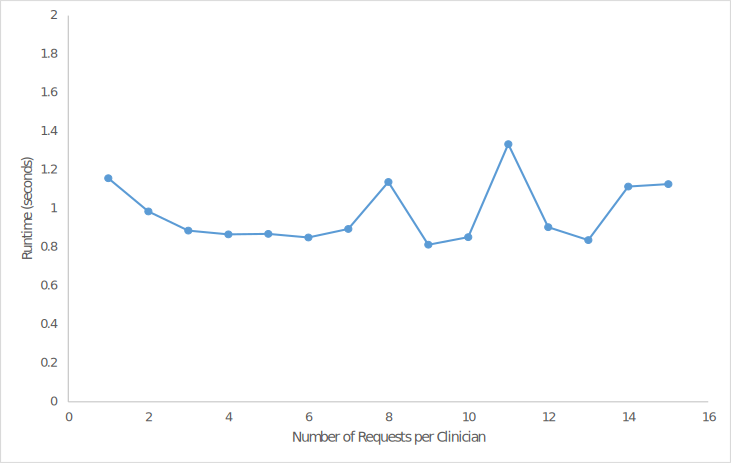
\includegraphics[scale=.5]{fig/runtime_requests} % JK: can you export this to PDF or SVG to avoid pixelation?
	\caption{Runtime of ILP solver with an increasing number of requests per clinician}
  \label{fig:runtime-requests}
  % JK: The trend here is a bit confusing, since I think you're trying to say
  %     that the runtime is not affected by the number of constraints,
  %     but there is noise in these results.
  %     I would re-run this 10-100 times and average the results so that (I expect)
  %     the mean trend is actually flat. You could (should) then also present the runtimes
  %     as box-plots to show that the trend is less than the variability.
\end{figure}

Figure~\ref{fig:runtime-blocks} presents the change in runtime when increasing
the number of 2-week blocks $B = \{26, 52, 78, 104\}$ in a department with 10
clinicians offering two services. There does not seem to be a strong effect on
runtime when we lengthen the time-horizon of the schedule, and in fact the
solver was able to find an optimal schedule for all time horizons within 3
seconds. % 'very reasonable amount of time" is vague. what is reasonable?
%better to give a range in value.

\begin{figure}[h]
	\centering
	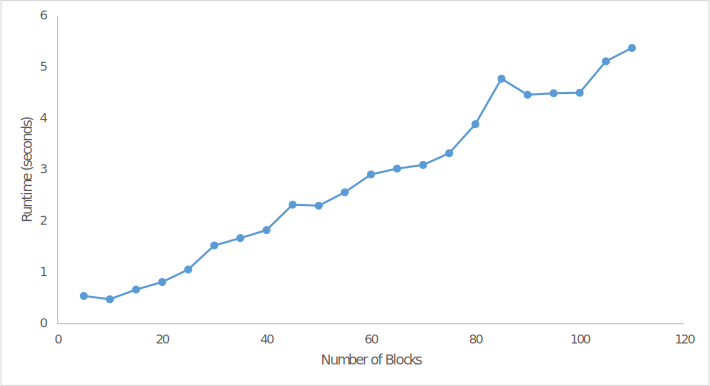
\includegraphics[scale=.5]{fig/runtime_blocks}
	\caption{Runtime of ILP solver with an increasing number of 2-week blocks}%
  \label{fig:runtime-blocks}
  % JK: same comment as above re. trends -- are you trying to show one?
  % JK: Thess figures could also possible be Figure 1. a) and b) 
\end{figure}

The effect of increasing the number of services %divisions %do you mean
%services?
on the runtime of the program is shown in Table~\ref{tbl:runtime-services-clinicians-comparison}. We executed the algorithm for
$S = \{1, 2, 3\}$ total services and $C = \{10, 20, 30, 50\}$ clinicians in
total across all services. For 2 concurrent services, a roster of 30 or more
clinicians becomes impractical to schedule, as searching for a solution required
over 24 hours. We saw similar issues for a roster of 20 or more clinicians
assigned to a division with 3 concurrent services. However, when relaxing the
NCB constraint, we saw a great improvement in runtime for divisions with 2 and 3
services, and we were able to generate a schedule with upwards of 50 clinicians
in under 1.5 seconds.  %what does division mean? do you mean services?

\begin{table}[h]
	\centering
	\begin{tabular}{|c|c||c|c||c|c|}
		\hline
		                                      &  \multicolumn{5}{c|}{Number of Services}  \\ \hline
		\makecell[l]{Number of \\ Clinicians} &  1   &    2    & 2 (CBA) &  3   & 3 (CBA) \\ \hline
		                 10                   & 0.16 &  0.74   &  0.16   & 1.40 &  0.23   \\ \hline
		                 20                   & 0.25 & 7468.86 &  0.32   &  -   &  0.43   \\ \hline
		                 30                   & 0.42 &    -    &  0.49   &  -   &  0.66   \\ \hline
		                 50                   & 0.62 &    -    &  0.82   &  -   &  1.14   \\ \hline
	\end{tabular}
	\caption{Comparison of program runtime (in seconds) for different number of services and total clinicians in the division. `-' indicates that a solution was not found after 24 hours. `CBA' indicates that \underline{c}onsecutive \underline{b}locks were \underline{a}llowed when generating these schedules.}
	\label{tbl:runtime-services-clinicians-comparison}%
\end{table}

	\section{Discussion}\label{sec:discussion}
	In this paper, we present a simple, yet flexible, integer linear programming
formulation to generate schedules for clinical departments at hospitals.
The challenge in applying ILP to the task of scheduling clinicians lies in the
computational complexity of finding an optimal solution. As the size of the
% JK: Is this a challenge of applying ILP? Or of the problem in general?
%     I got the impression that ILP was a nice way to overcome this problem.
scheduling problem grows, due to a larger roster of clinicians or more
complicated constraints, the time it takes to generate an optimal schedule may
grow exponentially.
%The challenge in applying such an approach to this task lies in the fact that
%ILP is an NP-hard problem. %specify what 'such an approach' and 'this task'
%are... the first part of the sentence was a bit hard to follow. Define what you
%mean by NP-hard problem and cite --> i.e. NP-hard = the following sentence
%about how time to optimal solution grows exponentially? if yes, then instead of
%'As such' - say 'That is,...or "An NP-hard problem means that..."
% JK: How come only "may"? Under what conditions?
As a result, the majority of approaches taken to create schedules for similar
scenarios tend to use heuristics in order to find an approximately optimal
solution in a shorter time~\cite{burke_state_2004}. %cite/reference
%statement (i.e. the 'vast majority'...) I can't remember if the introduction
%details the heuristics --> but if yes, then great. if no, then include that
%review of the prior literature here in discussion. I think as you said - the
%journals we are submitting to seem to have more of those details in the
%introduction.

%double-check all abbreviations have been defined. I would prefer limiting
%abbreviations to no more than 3 at most if possible. We are ok for word count
%in this paper :). 

We presented a formulation that includes both hard constraints to ensure the
schedule satisfies hospital and logistics requirements, and a multi-goal
objective function to satisfy soft constraints (work preferences of clinicians).
%Our formulation includes hard constraints to ensure the schedule satisfies
%hospital and logistics requirements. It also aims to satisfy the work
%preferences of clinicians in a clinical department by optimizing a multi-goal
%objective function. 
Although we restricted our application of the formulation to a set of
constraints for the particular needs of the case study (St.\ Michael's Hospital
Division of Infectious Diseases), our formulation can be adapted to various
clinical departments at different hospitals. The flexibility of our ILP allows
changing the number of services provided in a division, the length of a work
block, clinicians' preference for block to weekend adjacency as well as
clinicians' requests for time off.
% JK: Nice!

When comparing the optimal schedule generated by our tool to the
manually-created schedules at St.\ Michael's Hospital, we found that the ILP
formulation was always able to find an optimal schedule satisfying all required
hard constraints, unlike the manual schedule, which often did not satisfy all
constraints. Moreover, due to the multi-goal objective function in
the ILP, the algorithm was able to fulfill the majority of clinician
preferences and requests, more so than the manually-created schedule. These
observations reinforce the benefits of automated tools when generating schedules
in hospital departments to balance the workload of clinicians and improve the
service provided to patients. The use of automated tools alleviates the time
spent on designing the schedule by hand, and provides clinical departments with
a more fair distribution of work that helps improve the overall satisfaction of
both employees and patients~\cite{silvestro_evaluation_2000}.  % how the
%finding compares to the wider literature when automated compared to manual?
%What does it mean re: "so what" - human error in generating tools, etc. or
%challenges in heuristics used manually by people? include citations this last
%sentence in particular - what dos it reinforce exactly - what are the benefits?

In our simulations, we also found that increasing the number of requests per
clinician did not affect the runtime of the algorithm, highlighting the
flexibility of the tool to incorporate clinician preferences. Further, we saw
that the algorithm can accommodate an increase in time-horizon up to four years
with little impact on runtime, suggesting the algorithm can be used generate
schedules far in advance. One key limitation we identified was the sensitivity
of the runtime to larger numbers of services offered by a single department.
Such cases are unlikely to be encountered in the real-world because most
clinical departments tend to provide a single service or at most two services by
the same roster of clinicians [{\color{red}SM/Kevin, could you help with
	reference here?}]. One solution to mitigate the runtime issues created by a
larger number of services would be relaxing the constraints that prevent
assignment of consecutive blocks, followed by manual readjustment from the
generated schedule. %what do we mean by certain constraints? specify the other
%constraints?
Overall, our sensitivity analyses using simulated data provided reassurance that
the ILP formulation can be applied to schedule clinicians across real-world
variability between clinical departments. %SM - will look for reference and we
%can ask Kevin Gough too.
Next steps include expanding the generalizability of the tool beyond smaller
clinical departments to larger departments within and outside of health-care --
especially those that provide multiple services in parallel for patients and
other clients. 

	\section{Acknowledgements}\label{sec:acknowledgements}
	The authors are grateful to Julie Veitch for her contributions to testing and
designing the scheduling software. SM is supported by a Canadian Institutes of
Health Research New Investigator Award. DL conducted part of this project as a
Keenan Research Summer Student, Li Ka Shing Knowledge Institute, St. Michael's
Hospital, University of Toronto.

	\section{Funding}\label{sec:funding}
	The work was jointly funded by the Ontario Ministry of Science and Innovation Early Researcher Award Number ER17-13-043; the Division of Infectious Diseases, St.\ Michael's Hospital, University of Toronto; and the University of Toronto Work Study Program.
%SM - confirmed reviewed
	
	\bibliographystyle{unsrt}
	\bibliography{references}
\end{document}
